
% Default to the notebook output style

    


% Inherit from the specified cell style.




    
\documentclass[11pt]{article}

    
    
    \usepackage[T1]{fontenc}
    % Nicer default font (+ math font) than Computer Modern for most use cases
    \usepackage{mathpazo}
	\usepackage{float}
    % Basic figure setup, for now with no caption control since it's done
    % automatically by Pandoc (which extracts ![](path) syntax from Markdown).
    \usepackage{graphicx}
    % We will generate all images so they have a width \maxwidth. This means
    % that they will get their normal width if they fit onto the page, but
    % are scaled down if they would overflow the margins.
    \makeatletter
    \def\maxwidth{\ifdim\Gin@nat@width>\linewidth\linewidth
    \else\Gin@nat@width\fi}
    \makeatother
    \let\Oldincludegraphics\includegraphics
    % Set max figure width to be 80% of text width, for now hardcoded.
    \renewcommand{\includegraphics}[1]{\Oldincludegraphics[width=.8\maxwidth]{#1}}
    % Ensure that by default, figures have no caption (until we provide a
    % proper Figure object with a Caption API and a way to capture that
    % in the conversion process - todo).
    \usepackage{caption}
    \DeclareCaptionLabelFormat{nolabel}{}
    \captionsetup{labelformat=nolabel}

    \usepackage{adjustbox} % Used to constrain images to a maximum size 
    \usepackage{xcolor} % Allow colors to be defined
    \usepackage{enumerate} % Needed for markdown enumerations to work
    \usepackage{geometry} % Used to adjust the document margins
    \usepackage{amsmath} % Equations
    \usepackage{amssymb} % Equations
    \usepackage{textcomp} % defines textquotesingle
    % Hack from http://tex.stackexchange.com/a/47451/13684:
    \AtBeginDocument{%
        \def\PYZsq{\textquotesingle}% Upright quotes in Pygmentized code
    }
    \usepackage{upquote} % Upright quotes for verbatim code
    \usepackage{eurosym} % defines \euro
    \usepackage[mathletters]{ucs} % Extended unicode (utf-8) support
    \usepackage[utf8x]{inputenc} % Allow utf-8 characters in the tex document
    \usepackage{fancyvrb} % verbatim replacement that allows latex
    \usepackage{grffile} % extends the file name processing of package graphics 
                         % to support a larger range 
    % The hyperref package gives us a pdf with properly built
    % internal navigation ('pdf bookmarks' for the table of contents,
    % internal cross-reference links, web links for URLs, etc.)
    \usepackage{hyperref}
    \usepackage{longtable} % longtable support required by pandoc >1.10
    \usepackage{booktabs}  % table support for pandoc > 1.12.2
    \usepackage[inline]{enumitem} % IRkernel/repr support (it uses the enumerate* environment)
    \usepackage[normalem]{ulem} % ulem is needed to support strikethroughs (\sout)
                                % normalem makes italics be italics, not underlines
    \usepackage{mathrsfs}
    

    
    
    % Colors for the hyperref package
    \definecolor{urlcolor}{rgb}{0,.145,.698}
    \definecolor{linkcolor}{rgb}{.71,0.21,0.01}
    \definecolor{citecolor}{rgb}{.12,.54,.11}

    % ANSI colors
    \definecolor{ansi-black}{HTML}{3E424D}
    \definecolor{ansi-black-intense}{HTML}{282C36}
    \definecolor{ansi-red}{HTML}{E75C58}
    \definecolor{ansi-red-intense}{HTML}{B22B31}
    \definecolor{ansi-green}{HTML}{00A250}
    \definecolor{ansi-green-intense}{HTML}{007427}
    \definecolor{ansi-yellow}{HTML}{DDB62B}
    \definecolor{ansi-yellow-intense}{HTML}{B27D12}
    \definecolor{ansi-blue}{HTML}{208FFB}
    \definecolor{ansi-blue-intense}{HTML}{0065CA}
    \definecolor{ansi-magenta}{HTML}{D160C4}
    \definecolor{ansi-magenta-intense}{HTML}{A03196}
    \definecolor{ansi-cyan}{HTML}{60C6C8}
    \definecolor{ansi-cyan-intense}{HTML}{258F8F}
    \definecolor{ansi-white}{HTML}{C5C1B4}
    \definecolor{ansi-white-intense}{HTML}{A1A6B2}
    \definecolor{ansi-default-inverse-fg}{HTML}{FFFFFF}
    \definecolor{ansi-default-inverse-bg}{HTML}{000000}

    % commands and environments needed by pandoc snippets
    % extracted from the output of `pandoc -s`
    \providecommand{\tightlist}{%
      \setlength{\itemsep}{0pt}\setlength{\parskip}{0pt}}
    \DefineVerbatimEnvironment{Highlighting}{Verbatim}{commandchars=\\\{\}}
    % Add ',fontsize=\small' for more characters per line
    \newenvironment{Shaded}{}{}
    \newcommand{\KeywordTok}[1]{\textcolor[rgb]{0.00,0.44,0.13}{\textbf{{#1}}}}
    \newcommand{\DataTypeTok}[1]{\textcolor[rgb]{0.56,0.13,0.00}{{#1}}}
    \newcommand{\DecValTok}[1]{\textcolor[rgb]{0.25,0.63,0.44}{{#1}}}
    \newcommand{\BaseNTok}[1]{\textcolor[rgb]{0.25,0.63,0.44}{{#1}}}
    \newcommand{\FloatTok}[1]{\textcolor[rgb]{0.25,0.63,0.44}{{#1}}}
    \newcommand{\CharTok}[1]{\textcolor[rgb]{0.25,0.44,0.63}{{#1}}}
    \newcommand{\StringTok}[1]{\textcolor[rgb]{0.25,0.44,0.63}{{#1}}}
    \newcommand{\CommentTok}[1]{\textcolor[rgb]{0.38,0.63,0.69}{\textit{{#1}}}}
    \newcommand{\OtherTok}[1]{\textcolor[rgb]{0.00,0.44,0.13}{{#1}}}
    \newcommand{\AlertTok}[1]{\textcolor[rgb]{1.00,0.00,0.00}{\textbf{{#1}}}}
    \newcommand{\FunctionTok}[1]{\textcolor[rgb]{0.02,0.16,0.49}{{#1}}}
    \newcommand{\RegionMarkerTok}[1]{{#1}}
    \newcommand{\ErrorTok}[1]{\textcolor[rgb]{1.00,0.00,0.00}{\textbf{{#1}}}}
    \newcommand{\NormalTok}[1]{{#1}}
    
    % Additional commands for more recent versions of Pandoc
    \newcommand{\ConstantTok}[1]{\textcolor[rgb]{0.53,0.00,0.00}{{#1}}}
    \newcommand{\SpecialCharTok}[1]{\textcolor[rgb]{0.25,0.44,0.63}{{#1}}}
    \newcommand{\VerbatimStringTok}[1]{\textcolor[rgb]{0.25,0.44,0.63}{{#1}}}
    \newcommand{\SpecialStringTok}[1]{\textcolor[rgb]{0.73,0.40,0.53}{{#1}}}
    \newcommand{\ImportTok}[1]{{#1}}
    \newcommand{\DocumentationTok}[1]{\textcolor[rgb]{0.73,0.13,0.13}{\textit{{#1}}}}
    \newcommand{\AnnotationTok}[1]{\textcolor[rgb]{0.38,0.63,0.69}{\textbf{\textit{{#1}}}}}
    \newcommand{\CommentVarTok}[1]{\textcolor[rgb]{0.38,0.63,0.69}{\textbf{\textit{{#1}}}}}
    \newcommand{\VariableTok}[1]{\textcolor[rgb]{0.10,0.09,0.49}{{#1}}}
    \newcommand{\ControlFlowTok}[1]{\textcolor[rgb]{0.00,0.44,0.13}{\textbf{{#1}}}}
    \newcommand{\OperatorTok}[1]{\textcolor[rgb]{0.40,0.40,0.40}{{#1}}}
    \newcommand{\BuiltInTok}[1]{{#1}}
    \newcommand{\ExtensionTok}[1]{{#1}}
    \newcommand{\PreprocessorTok}[1]{\textcolor[rgb]{0.74,0.48,0.00}{{#1}}}
    \newcommand{\AttributeTok}[1]{\textcolor[rgb]{0.49,0.56,0.16}{{#1}}}
    \newcommand{\InformationTok}[1]{\textcolor[rgb]{0.38,0.63,0.69}{\textbf{\textit{{#1}}}}}
    \newcommand{\WarningTok}[1]{\textcolor[rgb]{0.38,0.63,0.69}{\textbf{\textit{{#1}}}}}
    
    
    % Define a nice break command that doesn't care if a line doesn't already
    % exist.
    \def\br{\hspace*{\fill} \\* }
    % Math Jax compatibility definitions
    \def\gt{>}
    \def\lt{<}
    \let\Oldtex\TeX
    \let\Oldlatex\LaTeX
    \renewcommand{\TeX}{\textrm{\Oldtex}}
    \renewcommand{\LaTeX}{\textrm{\Oldlatex}}
    % Document parameters
    % Document title
    \title{Assignment 2}
    \author{Jiarong Ye}
    
    
    
    
    

    % Pygments definitions
    
\makeatletter
\def\PY@reset{\let\PY@it=\relax \let\PY@bf=\relax%
    \let\PY@ul=\relax \let\PY@tc=\relax%
    \let\PY@bc=\relax \let\PY@ff=\relax}
\def\PY@tok#1{\csname PY@tok@#1\endcsname}
\def\PY@toks#1+{\ifx\relax#1\empty\else%
    \PY@tok{#1}\expandafter\PY@toks\fi}
\def\PY@do#1{\PY@bc{\PY@tc{\PY@ul{%
    \PY@it{\PY@bf{\PY@ff{#1}}}}}}}
\def\PY#1#2{\PY@reset\PY@toks#1+\relax+\PY@do{#2}}

\expandafter\def\csname PY@tok@w\endcsname{\def\PY@tc##1{\textcolor[rgb]{0.73,0.73,0.73}{##1}}}
\expandafter\def\csname PY@tok@c\endcsname{\let\PY@it=\textit\def\PY@tc##1{\textcolor[rgb]{0.25,0.50,0.50}{##1}}}
\expandafter\def\csname PY@tok@cp\endcsname{\def\PY@tc##1{\textcolor[rgb]{0.74,0.48,0.00}{##1}}}
\expandafter\def\csname PY@tok@k\endcsname{\let\PY@bf=\textbf\def\PY@tc##1{\textcolor[rgb]{0.00,0.50,0.00}{##1}}}
\expandafter\def\csname PY@tok@kp\endcsname{\def\PY@tc##1{\textcolor[rgb]{0.00,0.50,0.00}{##1}}}
\expandafter\def\csname PY@tok@kt\endcsname{\def\PY@tc##1{\textcolor[rgb]{0.69,0.00,0.25}{##1}}}
\expandafter\def\csname PY@tok@o\endcsname{\def\PY@tc##1{\textcolor[rgb]{0.40,0.40,0.40}{##1}}}
\expandafter\def\csname PY@tok@ow\endcsname{\let\PY@bf=\textbf\def\PY@tc##1{\textcolor[rgb]{0.67,0.13,1.00}{##1}}}
\expandafter\def\csname PY@tok@nb\endcsname{\def\PY@tc##1{\textcolor[rgb]{0.00,0.50,0.00}{##1}}}
\expandafter\def\csname PY@tok@nf\endcsname{\def\PY@tc##1{\textcolor[rgb]{0.00,0.00,1.00}{##1}}}
\expandafter\def\csname PY@tok@nc\endcsname{\let\PY@bf=\textbf\def\PY@tc##1{\textcolor[rgb]{0.00,0.00,1.00}{##1}}}
\expandafter\def\csname PY@tok@nn\endcsname{\let\PY@bf=\textbf\def\PY@tc##1{\textcolor[rgb]{0.00,0.00,1.00}{##1}}}
\expandafter\def\csname PY@tok@ne\endcsname{\let\PY@bf=\textbf\def\PY@tc##1{\textcolor[rgb]{0.82,0.25,0.23}{##1}}}
\expandafter\def\csname PY@tok@nv\endcsname{\def\PY@tc##1{\textcolor[rgb]{0.10,0.09,0.49}{##1}}}
\expandafter\def\csname PY@tok@no\endcsname{\def\PY@tc##1{\textcolor[rgb]{0.53,0.00,0.00}{##1}}}
\expandafter\def\csname PY@tok@nl\endcsname{\def\PY@tc##1{\textcolor[rgb]{0.63,0.63,0.00}{##1}}}
\expandafter\def\csname PY@tok@ni\endcsname{\let\PY@bf=\textbf\def\PY@tc##1{\textcolor[rgb]{0.60,0.60,0.60}{##1}}}
\expandafter\def\csname PY@tok@na\endcsname{\def\PY@tc##1{\textcolor[rgb]{0.49,0.56,0.16}{##1}}}
\expandafter\def\csname PY@tok@nt\endcsname{\let\PY@bf=\textbf\def\PY@tc##1{\textcolor[rgb]{0.00,0.50,0.00}{##1}}}
\expandafter\def\csname PY@tok@nd\endcsname{\def\PY@tc##1{\textcolor[rgb]{0.67,0.13,1.00}{##1}}}
\expandafter\def\csname PY@tok@s\endcsname{\def\PY@tc##1{\textcolor[rgb]{0.73,0.13,0.13}{##1}}}
\expandafter\def\csname PY@tok@sd\endcsname{\let\PY@it=\textit\def\PY@tc##1{\textcolor[rgb]{0.73,0.13,0.13}{##1}}}
\expandafter\def\csname PY@tok@si\endcsname{\let\PY@bf=\textbf\def\PY@tc##1{\textcolor[rgb]{0.73,0.40,0.53}{##1}}}
\expandafter\def\csname PY@tok@se\endcsname{\let\PY@bf=\textbf\def\PY@tc##1{\textcolor[rgb]{0.73,0.40,0.13}{##1}}}
\expandafter\def\csname PY@tok@sr\endcsname{\def\PY@tc##1{\textcolor[rgb]{0.73,0.40,0.53}{##1}}}
\expandafter\def\csname PY@tok@ss\endcsname{\def\PY@tc##1{\textcolor[rgb]{0.10,0.09,0.49}{##1}}}
\expandafter\def\csname PY@tok@sx\endcsname{\def\PY@tc##1{\textcolor[rgb]{0.00,0.50,0.00}{##1}}}
\expandafter\def\csname PY@tok@m\endcsname{\def\PY@tc##1{\textcolor[rgb]{0.40,0.40,0.40}{##1}}}
\expandafter\def\csname PY@tok@gh\endcsname{\let\PY@bf=\textbf\def\PY@tc##1{\textcolor[rgb]{0.00,0.00,0.50}{##1}}}
\expandafter\def\csname PY@tok@gu\endcsname{\let\PY@bf=\textbf\def\PY@tc##1{\textcolor[rgb]{0.50,0.00,0.50}{##1}}}
\expandafter\def\csname PY@tok@gd\endcsname{\def\PY@tc##1{\textcolor[rgb]{0.63,0.00,0.00}{##1}}}
\expandafter\def\csname PY@tok@gi\endcsname{\def\PY@tc##1{\textcolor[rgb]{0.00,0.63,0.00}{##1}}}
\expandafter\def\csname PY@tok@gr\endcsname{\def\PY@tc##1{\textcolor[rgb]{1.00,0.00,0.00}{##1}}}
\expandafter\def\csname PY@tok@ge\endcsname{\let\PY@it=\textit}
\expandafter\def\csname PY@tok@gs\endcsname{\let\PY@bf=\textbf}
\expandafter\def\csname PY@tok@gp\endcsname{\let\PY@bf=\textbf\def\PY@tc##1{\textcolor[rgb]{0.00,0.00,0.50}{##1}}}
\expandafter\def\csname PY@tok@go\endcsname{\def\PY@tc##1{\textcolor[rgb]{0.53,0.53,0.53}{##1}}}
\expandafter\def\csname PY@tok@gt\endcsname{\def\PY@tc##1{\textcolor[rgb]{0.00,0.27,0.87}{##1}}}
\expandafter\def\csname PY@tok@err\endcsname{\def\PY@bc##1{\setlength{\fboxsep}{0pt}\fcolorbox[rgb]{1.00,0.00,0.00}{1,1,1}{\strut ##1}}}
\expandafter\def\csname PY@tok@kc\endcsname{\let\PY@bf=\textbf\def\PY@tc##1{\textcolor[rgb]{0.00,0.50,0.00}{##1}}}
\expandafter\def\csname PY@tok@kd\endcsname{\let\PY@bf=\textbf\def\PY@tc##1{\textcolor[rgb]{0.00,0.50,0.00}{##1}}}
\expandafter\def\csname PY@tok@kn\endcsname{\let\PY@bf=\textbf\def\PY@tc##1{\textcolor[rgb]{0.00,0.50,0.00}{##1}}}
\expandafter\def\csname PY@tok@kr\endcsname{\let\PY@bf=\textbf\def\PY@tc##1{\textcolor[rgb]{0.00,0.50,0.00}{##1}}}
\expandafter\def\csname PY@tok@bp\endcsname{\def\PY@tc##1{\textcolor[rgb]{0.00,0.50,0.00}{##1}}}
\expandafter\def\csname PY@tok@fm\endcsname{\def\PY@tc##1{\textcolor[rgb]{0.00,0.00,1.00}{##1}}}
\expandafter\def\csname PY@tok@vc\endcsname{\def\PY@tc##1{\textcolor[rgb]{0.10,0.09,0.49}{##1}}}
\expandafter\def\csname PY@tok@vg\endcsname{\def\PY@tc##1{\textcolor[rgb]{0.10,0.09,0.49}{##1}}}
\expandafter\def\csname PY@tok@vi\endcsname{\def\PY@tc##1{\textcolor[rgb]{0.10,0.09,0.49}{##1}}}
\expandafter\def\csname PY@tok@vm\endcsname{\def\PY@tc##1{\textcolor[rgb]{0.10,0.09,0.49}{##1}}}
\expandafter\def\csname PY@tok@sa\endcsname{\def\PY@tc##1{\textcolor[rgb]{0.73,0.13,0.13}{##1}}}
\expandafter\def\csname PY@tok@sb\endcsname{\def\PY@tc##1{\textcolor[rgb]{0.73,0.13,0.13}{##1}}}
\expandafter\def\csname PY@tok@sc\endcsname{\def\PY@tc##1{\textcolor[rgb]{0.73,0.13,0.13}{##1}}}
\expandafter\def\csname PY@tok@dl\endcsname{\def\PY@tc##1{\textcolor[rgb]{0.73,0.13,0.13}{##1}}}
\expandafter\def\csname PY@tok@s2\endcsname{\def\PY@tc##1{\textcolor[rgb]{0.73,0.13,0.13}{##1}}}
\expandafter\def\csname PY@tok@sh\endcsname{\def\PY@tc##1{\textcolor[rgb]{0.73,0.13,0.13}{##1}}}
\expandafter\def\csname PY@tok@s1\endcsname{\def\PY@tc##1{\textcolor[rgb]{0.73,0.13,0.13}{##1}}}
\expandafter\def\csname PY@tok@mb\endcsname{\def\PY@tc##1{\textcolor[rgb]{0.40,0.40,0.40}{##1}}}
\expandafter\def\csname PY@tok@mf\endcsname{\def\PY@tc##1{\textcolor[rgb]{0.40,0.40,0.40}{##1}}}
\expandafter\def\csname PY@tok@mh\endcsname{\def\PY@tc##1{\textcolor[rgb]{0.40,0.40,0.40}{##1}}}
\expandafter\def\csname PY@tok@mi\endcsname{\def\PY@tc##1{\textcolor[rgb]{0.40,0.40,0.40}{##1}}}
\expandafter\def\csname PY@tok@il\endcsname{\def\PY@tc##1{\textcolor[rgb]{0.40,0.40,0.40}{##1}}}
\expandafter\def\csname PY@tok@mo\endcsname{\def\PY@tc##1{\textcolor[rgb]{0.40,0.40,0.40}{##1}}}
\expandafter\def\csname PY@tok@ch\endcsname{\let\PY@it=\textit\def\PY@tc##1{\textcolor[rgb]{0.25,0.50,0.50}{##1}}}
\expandafter\def\csname PY@tok@cm\endcsname{\let\PY@it=\textit\def\PY@tc##1{\textcolor[rgb]{0.25,0.50,0.50}{##1}}}
\expandafter\def\csname PY@tok@cpf\endcsname{\let\PY@it=\textit\def\PY@tc##1{\textcolor[rgb]{0.25,0.50,0.50}{##1}}}
\expandafter\def\csname PY@tok@c1\endcsname{\let\PY@it=\textit\def\PY@tc##1{\textcolor[rgb]{0.25,0.50,0.50}{##1}}}
\expandafter\def\csname PY@tok@cs\endcsname{\let\PY@it=\textit\def\PY@tc##1{\textcolor[rgb]{0.25,0.50,0.50}{##1}}}

\def\PYZbs{\char`\\}
\def\PYZus{\char`\_}
\def\PYZob{\char`\{}
\def\PYZcb{\char`\}}
\def\PYZca{\char`\^}
\def\PYZam{\char`\&}
\def\PYZlt{\char`\<}
\def\PYZgt{\char`\>}
\def\PYZsh{\char`\#}
\def\PYZpc{\char`\%}
\def\PYZdl{\char`\$}
\def\PYZhy{\char`\-}
\def\PYZsq{\char`\'}
\def\PYZdq{\char`\"}
\def\PYZti{\char`\~}
% for compatibility with earlier versions
\def\PYZat{@}
\def\PYZlb{[}
\def\PYZrb{]}
\makeatother


    % Exact colors from NB
    \definecolor{incolor}{rgb}{0.0, 0.0, 0.5}
    \definecolor{outcolor}{rgb}{0.545, 0.0, 0.0}



    
    % Prevent overflowing lines due to hard-to-break entities
    \sloppy 
    % Setup hyperref package
    \hypersetup{
      breaklinks=true,  % so long urls are correctly broken across lines
      colorlinks=true,
      urlcolor=urlcolor,
      linkcolor=linkcolor,
      citecolor=citecolor,
      }
    % Slightly bigger margins than the latex defaults
    
    \geometry{verbose,tmargin=1in,bmargin=1in,lmargin=1in,rmargin=1in}
    
    

    \begin{document}
    
    
    \maketitle
    
    

    
    \subsection*{Import packages}\label{import-packages}

    \begin{Verbatim}[commandchars=\\\{\}]
{\color{incolor}In [{\color{incolor}117}]:} \PY{k+kn}{import} \PY{n+nn}{redis}
          \PY{k+kn}{from} \PY{n+nn}{urllib}\PY{n+nn}{.}\PY{n+nn}{request} \PY{k}{import} \PY{n}{urlopen}
          \PY{k+kn}{import} \PY{n+nn}{pandas} \PY{k}{as} \PY{n+nn}{pd}
          \PY{k+kn}{import} \PY{n+nn}{re}
          \PY{k+kn}{from} \PY{n+nn}{bs4} \PY{k}{import} \PY{n}{BeautifulSoup}
\end{Verbatim}

    \subsection*{scrape car retail information from a chosen car dealer
website}\label{scrape-car-retail-information-from-a-chosen-car-dealer-website}

    \paragraph{Titles}\label{titles}

    \begin{Verbatim}[commandchars=\\\{\}]
{\color{incolor}In [{\color{incolor}245}]:} \PY{n}{url} \PY{o}{=} \PY{l+s+s1}{\PYZsq{}}\PY{l+s+s1}{http://www.statecollege.com/auto/dealers/stocker\PYZhy{}chevrolet,9803/}\PY{l+s+s1}{\PYZsq{}}
          \PY{n}{page} \PY{o}{=} \PY{n}{urlopen}\PY{p}{(}\PY{n}{url}\PY{o}{=}\PY{n}{url}\PY{p}{)}
          \PY{n}{soup} \PY{o}{=} \PY{n}{BeautifulSoup}\PY{p}{(}\PY{n}{page}\PY{p}{,} \PY{l+s+s1}{\PYZsq{}}\PY{l+s+s1}{html.parser}\PY{l+s+s1}{\PYZsq{}}\PY{p}{)}
          \PY{n}{titles} \PY{o}{=} \PY{n}{soup}\PY{o}{.}\PY{n}{findAll}\PY{p}{(}\PY{l+s+s1}{\PYZsq{}}\PY{l+s+s1}{strong}\PY{l+s+s1}{\PYZsq{}}\PY{p}{,} \PY{p}{\PYZob{}}\PY{l+s+s2}{\PYZdq{}}\PY{l+s+s2}{class}\PY{l+s+s2}{\PYZdq{}}\PY{p}{:} \PY{l+s+s2}{\PYZdq{}}\PY{l+s+s2}{title}\PY{l+s+s2}{\PYZdq{}}\PY{p}{\PYZcb{}}\PY{p}{)}
          \PY{n}{titles\PYZus{}df} \PY{o}{=} \PY{n}{pd}\PY{o}{.}\PY{n}{DataFrame}\PY{p}{(}\PY{n+nb}{list}\PY{p}{(}\PY{n+nb}{map}\PY{p}{(}\PY{k}{lambda} \PY{n}{x}\PY{p}{:} \PY{n}{x}\PY{o}{.}\PY{n}{getText}\PY{p}{(}\PY{p}{)}\PY{p}{,} \PY{n}{titles}\PY{p}{)}\PY{p}{)}\PY{p}{,} \PY{n}{columns}\PY{o}{=}\PY{p}{[}\PY{l+s+s1}{\PYZsq{}}\PY{l+s+s1}{Title}\PY{l+s+s1}{\PYZsq{}}\PY{p}{]}\PY{p}{)}
\end{Verbatim}

    \paragraph{Embedded urls}\label{embedded-urls}

    \begin{Verbatim}[commandchars=\\\{\}]
{\color{incolor}In [{\color{incolor}246}]:} \PY{n}{urls\PYZus{}df} \PY{o}{=} \PY{n}{pd}\PY{o}{.}\PY{n}{DataFrame}\PY{p}{(}\PY{p}{[}\PY{l+s+s1}{\PYZsq{}}\PY{l+s+s1}{http://www.statecollege.com/}\PY{l+s+s1}{\PYZsq{}}\PY{o}{+} \PY{n}{a}\PY{p}{[}\PY{l+s+s1}{\PYZsq{}}\PY{l+s+s1}{href}\PY{l+s+s1}{\PYZsq{}}\PY{p}{]} \PY{k}{for} \PY{n}{i} \PY{o+ow}{in} \PY{n}{soup}\PY{o}{.}\PY{n}{findAll}\PY{p}{(}\PY{l+s+s1}{\PYZsq{}}\PY{l+s+s1}{td}\PY{l+s+s1}{\PYZsq{}}\PY{p}{,} \PY{p}{\PYZob{}}\PY{l+s+s1}{\PYZsq{}}\PY{l+s+s1}{align}\PY{l+s+s1}{\PYZsq{}}\PY{p}{:} \PY{l+s+s1}{\PYZsq{}}\PY{l+s+s1}{left}\PY{l+s+s1}{\PYZsq{}}\PY{p}{\PYZcb{}}\PY{p}{)} \PY{k}{for} \PY{n}{a} \PY{o+ow}{in} \PY{n}{i}\PY{o}{.}\PY{n}{findAll}\PY{p}{(}\PY{l+s+s1}{\PYZsq{}}\PY{l+s+s1}{a}\PY{l+s+s1}{\PYZsq{}}\PY{p}{,} \PY{n}{href}\PY{o}{=}\PY{k+kc}{True}\PY{p}{)}\PY{p}{]}\PY{p}{,} \PY{n}{columns}\PY{o}{=}\PY{p}{[}\PY{l+s+s1}{\PYZsq{}}\PY{l+s+s1}{urls}\PY{l+s+s1}{\PYZsq{}}\PY{p}{]}\PY{p}{)}
\end{Verbatim}

    \paragraph{Addresses, phones of sellers \& descriptions of
cars}\label{addresses-phones-of-sellers-descriptions-of-cars}

    \begin{Verbatim}[commandchars=\\\{\}]
{\color{incolor}In [{\color{incolor}247}]:} \PY{n}{addresses} \PY{o}{=} \PY{p}{[}\PY{p}{]}
          \PY{n}{phones} \PY{o}{=} \PY{p}{[}\PY{p}{]}
          \PY{n}{descriptions} \PY{o}{=} \PY{p}{[}\PY{p}{]}
          \PY{k}{for} \PY{n}{url} \PY{o+ow}{in} \PY{n}{urls\PYZus{}df}\PY{o}{.}\PY{n}{values}\PY{p}{:}
              \PY{n}{page} \PY{o}{=} \PY{n}{urlopen}\PY{p}{(}\PY{n}{url}\PY{o}{=}\PY{n}{url}\PY{p}{[}\PY{l+m+mi}{0}\PY{p}{]}\PY{p}{)}
              \PY{n}{soup} \PY{o}{=} \PY{n}{BeautifulSoup}\PY{p}{(}\PY{n}{page}\PY{p}{,} \PY{l+s+s1}{\PYZsq{}}\PY{l+s+s1}{html.parser}\PY{l+s+s1}{\PYZsq{}}\PY{p}{)}
              \PY{k}{for} \PY{n}{address} \PY{o+ow}{in} \PY{n}{soup}\PY{o}{.}\PY{n}{findAll}\PY{p}{(}\PY{l+s+s1}{\PYZsq{}}\PY{l+s+s1}{p}\PY{l+s+s1}{\PYZsq{}}\PY{p}{,} \PY{p}{\PYZob{}}\PY{l+s+s1}{\PYZsq{}}\PY{l+s+s1}{class}\PY{l+s+s1}{\PYZsq{}}\PY{p}{:} \PY{l+s+s1}{\PYZsq{}}\PY{l+s+s1}{business\PYZus{}address\PYZus{}address}\PY{l+s+s1}{\PYZsq{}}\PY{p}{\PYZcb{}}\PY{p}{)}\PY{p}{:}
                  \PY{n}{addresses}\PY{o}{.}\PY{n}{append}\PY{p}{(}\PY{n}{re}\PY{o}{.}\PY{n}{sub}\PY{p}{(}\PY{l+s+s1}{\PYZsq{}}\PY{l+s+s1}{\PYZbs{}}\PY{l+s+s1}{s+}\PY{l+s+s1}{\PYZsq{}}\PY{p}{,} \PY{l+s+s1}{\PYZsq{}}\PY{l+s+s1}{ }\PY{l+s+s1}{\PYZsq{}}\PY{p}{,} \PY{n}{address}\PY{o}{.}\PY{n}{getText}\PY{p}{(}\PY{p}{)}\PY{o}{.}\PY{n}{replace}\PY{p}{(}\PY{l+s+s1}{\PYZsq{}}\PY{l+s+se}{\PYZbs{}n}\PY{l+s+s1}{\PYZsq{}}\PY{p}{,} \PY{l+s+s1}{\PYZsq{}}\PY{l+s+s1}{\PYZsq{}}\PY{p}{)}\PY{p}{)}\PY{p}{)}
              \PY{k}{for} \PY{n}{phone} \PY{o+ow}{in} \PY{n}{soup}\PY{o}{.}\PY{n}{find}\PY{p}{(}\PY{l+s+s1}{\PYZsq{}}\PY{l+s+s1}{p}\PY{l+s+s1}{\PYZsq{}}\PY{p}{,} \PY{p}{\PYZob{}}\PY{l+s+s1}{\PYZsq{}}\PY{l+s+s1}{class}\PY{l+s+s1}{\PYZsq{}}\PY{p}{:} \PY{l+s+s1}{\PYZsq{}}\PY{l+s+s1}{business\PYZus{}address\PYZus{}phone}\PY{l+s+s1}{\PYZsq{}}\PY{p}{\PYZcb{}}\PY{p}{)}\PY{p}{:}
                  \PY{n}{phones}\PY{o}{.}\PY{n}{append}\PY{p}{(}\PY{n}{phone}\PY{p}{)}
              \PY{k}{for} \PY{n}{i}\PY{p}{,} \PY{n}{c} \PY{o+ow}{in} \PY{n+nb}{enumerate}\PY{p}{(}\PY{n}{soup}\PY{o}{.}\PY{n}{findAll}\PY{p}{(}\PY{l+s+s1}{\PYZsq{}}\PY{l+s+s1}{p}\PY{l+s+s1}{\PYZsq{}}\PY{p}{)}\PY{p}{)}\PY{p}{:}
                  \PY{k}{if} \PY{n}{i}\PY{o}{==}\PY{l+m+mi}{5}\PY{p}{:}
                      \PY{n}{descriptions}\PY{o}{.}\PY{n}{append}\PY{p}{(}\PY{n}{c}\PY{o}{.}\PY{n}{getText}\PY{p}{(}\PY{p}{)}\PY{p}{)}
          \PY{n}{address\PYZus{}df} \PY{o}{=} \PY{n}{pd}\PY{o}{.}\PY{n}{DataFrame}\PY{p}{(}\PY{n}{addresses}\PY{p}{,} \PY{n}{columns}\PY{o}{=}\PY{p}{[}\PY{l+s+s1}{\PYZsq{}}\PY{l+s+s1}{address}\PY{l+s+s1}{\PYZsq{}}\PY{p}{]}\PY{p}{)}
          \PY{n}{phones\PYZus{}df} \PY{o}{=} \PY{n}{pd}\PY{o}{.}\PY{n}{DataFrame}\PY{p}{(}\PY{n}{phones}\PY{p}{,} \PY{n}{columns}\PY{o}{=}\PY{p}{[}\PY{l+s+s1}{\PYZsq{}}\PY{l+s+s1}{phone}\PY{l+s+s1}{\PYZsq{}}\PY{p}{]}\PY{p}{)}
          \PY{n}{descriptions\PYZus{}df} \PY{o}{=} \PY{n}{pd}\PY{o}{.}\PY{n}{DataFrame}\PY{p}{(}\PY{n}{descriptions}\PY{p}{,} \PY{n}{columns}\PY{o}{=}\PY{p}{[}\PY{l+s+s1}{\PYZsq{}}\PY{l+s+s1}{description}\PY{l+s+s1}{\PYZsq{}}\PY{p}{]}\PY{p}{)}
\end{Verbatim}

    \paragraph{Other attributes}\label{other-attributes}

    \begin{Verbatim}[commandchars=\\\{\}]
{\color{incolor}In [{\color{incolor}248}]:} \PY{n}{tables} \PY{o}{=} \PY{p}{[}\PY{p}{]}
          \PY{k}{for} \PY{n}{url} \PY{o+ow}{in} \PY{n}{urls\PYZus{}df}\PY{o}{.}\PY{n}{values}\PY{p}{:}
              \PY{n}{page} \PY{o}{=} \PY{n}{urlopen}\PY{p}{(}\PY{n}{url}\PY{o}{=}\PY{n}{url}\PY{p}{[}\PY{l+m+mi}{0}\PY{p}{]}\PY{p}{)}
              \PY{n}{soup} \PY{o}{=} \PY{n}{BeautifulSoup}\PY{p}{(}\PY{n}{page}\PY{p}{,} \PY{l+s+s1}{\PYZsq{}}\PY{l+s+s1}{html.parser}\PY{l+s+s1}{\PYZsq{}}\PY{p}{)}
              \PY{k}{for} \PY{n}{table} \PY{o+ow}{in} \PY{n}{soup}\PY{o}{.}\PY{n}{findAll}\PY{p}{(}\PY{l+s+s1}{\PYZsq{}}\PY{l+s+s1}{table}\PY{l+s+s1}{\PYZsq{}}\PY{p}{,} \PY{p}{\PYZob{}}\PY{l+s+s1}{\PYZsq{}}\PY{l+s+s1}{class}\PY{l+s+s1}{\PYZsq{}}\PY{p}{:} \PY{l+s+s1}{\PYZsq{}}\PY{l+s+s1}{auto\PYZus{}detail\PYZus{}data\PYZus{}table}\PY{l+s+s1}{\PYZsq{}}\PY{p}{\PYZcb{}}\PY{p}{)}\PY{p}{:}
                  \PY{n}{table} \PY{o}{=} \PY{n}{pd}\PY{o}{.}\PY{n}{read\PYZus{}html}\PY{p}{(}\PY{n+nb}{str}\PY{p}{(}\PY{n}{table}\PY{p}{)}\PY{p}{)} 
                  \PY{n}{tables}\PY{o}{.}\PY{n}{append}\PY{p}{(}\PY{n}{table}\PY{p}{)}
\end{Verbatim}

    \begin{Verbatim}[commandchars=\\\{\}]
{\color{incolor}In [{\color{incolor}249}]:} \PY{n}{attributes} \PY{o}{=} \PY{p}{[}\PY{l+s+s1}{\PYZsq{}}\PY{l+s+s1}{Year}\PY{l+s+s1}{\PYZsq{}}\PY{p}{,} \PY{l+s+s1}{\PYZsq{}}\PY{l+s+s1}{Mileage}\PY{l+s+s1}{\PYZsq{}}\PY{p}{,} \PY{l+s+s1}{\PYZsq{}}\PY{l+s+s1}{Make}\PY{l+s+s1}{\PYZsq{}}\PY{p}{,} \PY{l+s+s1}{\PYZsq{}}\PY{l+s+s1}{Model}\PY{l+s+s1}{\PYZsq{}}\PY{p}{,} \PY{l+s+s1}{\PYZsq{}}\PY{l+s+s1}{Trim}\PY{l+s+s1}{\PYZsq{}}\PY{p}{,} \PY{l+s+s1}{\PYZsq{}}\PY{l+s+s1}{Style}\PY{l+s+s1}{\PYZsq{}}\PY{p}{,} \PY{l+s+s1}{\PYZsq{}}\PY{l+s+s1}{Engine}\PY{l+s+s1}{\PYZsq{}}\PY{p}{,} \PY{l+s+s1}{\PYZsq{}}\PY{l+s+s1}{Exterior Color}\PY{l+s+s1}{\PYZsq{}}\PY{p}{,} \PY{l+s+s1}{\PYZsq{}}\PY{l+s+s1}{Interior Color}\PY{l+s+s1}{\PYZsq{}}\PY{p}{,} \PY{l+s+s1}{\PYZsq{}}\PY{l+s+s1}{VIN}\PY{l+s+s1}{\PYZsq{}}\PY{p}{,} \PY{l+s+s1}{\PYZsq{}}\PY{l+s+s1}{Stock \PYZsh{}}\PY{l+s+s1}{\PYZsq{}}\PY{p}{]}
          \PY{n}{attributes\PYZus{}dict} \PY{o}{=} \PY{p}{\PYZob{}}\PY{p}{\PYZcb{}}
          \PY{k}{for} \PY{n}{i} \PY{o+ow}{in} \PY{n}{attributes}\PY{p}{:}
              \PY{n}{attributes\PYZus{}dict}\PY{p}{[}\PY{n}{i}\PY{p}{]} \PY{o}{=} \PY{p}{[}\PY{p}{]}
          \PY{k}{for} \PY{n}{table} \PY{o+ow}{in} \PY{n}{tables}\PY{p}{:}
              \PY{n}{table} \PY{o}{=} \PY{n}{table}\PY{p}{[}\PY{l+m+mi}{0}\PY{p}{]}
              \PY{k}{for} \PY{n}{attribute} \PY{o+ow}{in} \PY{n}{attributes}\PY{p}{:}
                  \PY{n}{attributes\PYZus{}dict}\PY{p}{[}\PY{n}{attribute}\PY{p}{]}\PY{o}{.}\PY{n}{append}\PY{p}{(}\PY{n}{table}\PY{p}{[}\PY{n}{table}\PY{o}{.}\PY{n}{iloc}\PY{p}{[}\PY{p}{:}\PY{p}{,} \PY{l+m+mi}{0}\PY{p}{]}\PY{o}{==}\PY{n}{attribute}\PY{o}{+}\PY{l+s+s1}{\PYZsq{}}\PY{l+s+s1}{:}\PY{l+s+s1}{\PYZsq{}}\PY{p}{]}\PY{o}{.}\PY{n}{iloc}\PY{p}{[}\PY{p}{:}\PY{p}{,} \PY{l+m+mi}{1}\PY{p}{]}\PY{o}{.}\PY{n}{values}\PY{p}{[}\PY{l+m+mi}{0}\PY{p}{]}\PY{p}{)}
          \PY{n}{dataset} \PY{o}{=} \PY{n}{pd}\PY{o}{.}\PY{n}{concat}\PY{p}{(}\PY{p}{[}\PY{n}{titles\PYZus{}df}\PY{p}{,} \PY{n}{address\PYZus{}df}\PY{p}{,} \PY{n}{phones\PYZus{}df}\PY{p}{,} \PY{n}{pd}\PY{o}{.}\PY{n}{DataFrame}\PY{p}{(}\PY{n}{attributes\PYZus{}dict}\PY{p}{)}\PY{p}{,} \PY{n}{descriptions\PYZus{}df}\PY{p}{]}\PY{p}{,} \PY{n}{axis}\PY{o}{=}\PY{l+m+mi}{1}\PY{p}{)}
\end{Verbatim}

    \paragraph{Combine all attributes}\label{combine-all-attributes}

    \begin{Verbatim}[commandchars=\\\{\}]
{\color{incolor}In [{\color{incolor}257}]:} \PY{n}{dataset}
\end{Verbatim}

\begin{Verbatim}[commandchars=\\\{\}]
{\color{outcolor}Out[{\color{outcolor}257}]:}                            Title                                    address  \textbackslash{}
          0            2014 Subaru Outback   701 Benner Pike State College PA, 16801    
          1       2013 Subaru XV Crosstrek   701 Benner Pike State College PA, 16801    
          2           2014 Chevrolet Cruze   701 Benner Pike State College PA, 16801    
          3          2015 Chevrolet Malibu   701 Benner Pike State College PA, 16801    
          4  2015 Chevrolet Silverado 1500   701 Benner Pike State College PA, 16801    
          5  2016 Chevrolet Malibu Limited   701 Benner Pike State College PA, 16801    
          6           2016 Subaru Forester   701 Benner Pike State College PA, 16801    
          7  2015 Chevrolet Silverado 1500   701 Benner Pike State College PA, 16801    
          8             2017 Subaru Legacy   701 Benner Pike State College PA, 16801    
          9            2017 Subaru Outback   701 Benner Pike State College PA, 16801    
          
                      phone  Year Mileage       Make           Model          Trim  \textbackslash{}
          0  (866) 235-0270  2014   75655     Subaru         Outback  2.5i Premium   
          1  (866) 235-0270  2013   69331     Subaru    XV Crosstrek       Premium   
          2  (866) 235-0270  2014   61147  Chevrolet           Cruze            LS   
          3  (866) 235-0270  2015   25757  Chevrolet          Malibu            LS   
          4  (866) 235-0270  2015   41869  Chevrolet  Silverado 1500  High Country   
          5  (866) 235-0270  2016   52582  Chevrolet  Malibu Limited            LS   
          6  (866) 235-0270  2016   16994     Subaru        Forester          2.5i   
          7  (866) 235-0270  2015   49503  Chevrolet  Silverado 1500            LT   
          8  (866) 235-0270  2017       2     Subaru          Legacy       Limited   
          9  (866) 235-0270  2017       3     Subaru         Outback       Limited   
          
                       Style Engine        Exterior Color        Interior Color  \textbackslash{}
          0    Sport Utility    4 -  Twilight Blue Metall                 Black   
          1    Station Wagon    4 -  Tangerine Orange Pea                 Black   
          2          4dr Car    4 -  Atlantis Blue Metall  Jet Black/Medium Tit   
          3          4dr Car    4 -   Ashen Gray Metallic    Jet Black/Titanium   
          4  Crew Cab Pickup    8 -    Deep Ruby Metallic                Saddle   
          5          4dr Car    4 -  Champagne Silver Met    Jet Black/Titanium   
          6    Sport Utility    4 -   Ice Silver Metallic                 Black   
          7  Crew Cab Pickup    8 -          Summit White             Jet Black   
          8          4dr Car    6 -     Tungsten Metallic            Warm Ivory   
          9    Sport Utility    4 -  Twilight Blue Metall           Slate Black   
          
                           VIN  Stock \#  \textbackslash{}
          0  4S4BRBCC4E3219562  606614A   
          1  JF2GPACCXD1843307  204842B   
          2  1G1PA5SG4E7343131  204275A   
          3  1G11B5SL2FF313357  204597A   
          4  3GCUKTEC9FG401065  204778A   
          5  1G11B5SAXGF135777   15498A   
          6  JF2SJAAC3GG451169  606499A   
          7  3GCUKREC9FG459437  204882A   
          8  4S3BNEN6XH3029939   604992   
          9  4S4BSANC0H3391975   605565   
          
                                                   description  
          0  CARFAX One-Owner. Clean CARFAX. Blue 2014 Suba{\ldots}  
          1  Clean CARFAX. Orange 2013 Subaru XV Crosstrek {\ldots}  
          2  CARFAX One-Owner. Clean CARFAX. Blue 2014 Chev{\ldots}  
          3  CARFAX One-Owner. Clean CARFAX. Grey 2015 Chev{\ldots}  
          4  CARFAX One-Owner. Clean CARFAX. Burgundy 2015 {\ldots}  
          5  CARFAX One-Owner. Gold 2016 Chevrolet Malibu L{\ldots}  
          6  CARFAX One-Owner. Clean CARFAX. Ice Silver Met{\ldots}  
          7  CARFAX One-Owner. Clean CARFAX. White 2015 Che{\ldots}  
          8  \$750 off MSRP!We at Stocker Chevrolet apprecia{\ldots}  
          9  We at Stocker Chevrolet appreciate your time a{\ldots}  
\end{Verbatim}
            
            
            
    \paragraph{Insert data into Redis}\label{insert-data-into-redis}

    \begin{Verbatim}[commandchars=\\\{\}]
{\color{incolor}In [{\color{incolor}260}]:} \PY{n}{seller\PYZus{}address}\PY{o}{=}\PY{l+s+s1}{\PYZsq{}}\PY{l+s+s1}{\PYZsq{}}
          \PY{n}{seller\PYZus{}phone}\PY{o}{=}\PY{l+s+s1}{\PYZsq{}}\PY{l+s+s1}{\PYZsq{}}
          \PY{k}{for} \PY{n}{idx}\PY{p}{,} \PY{n}{t} \PY{o+ow}{in} \PY{n+nb}{enumerate}\PY{p}{(}\PY{n}{dataset}\PY{o}{.}\PY{n}{values}\PY{p}{)}\PY{p}{:}
              \PY{n}{r} \PY{o}{=} \PY{n}{redis}\PY{o}{.}\PY{n}{StrictRedis}\PY{p}{(}\PY{n}{host}\PY{o}{=}\PY{l+s+s1}{\PYZsq{}}\PY{l+s+s1}{localhost}\PY{l+s+s1}{\PYZsq{}}\PY{p}{,} \PY{n}{port}\PY{o}{=}\PY{l+m+mi}{6379}\PY{p}{,} \PY{n}{db}\PY{o}{=}\PY{n}{idx}\PY{p}{)}
              \PY{k}{for} \PY{n}{i}\PY{p}{,} \PY{n}{attribute} \PY{o+ow}{in} \PY{n+nb}{enumerate}\PY{p}{(}\PY{n}{dataset}\PY{o}{.}\PY{n}{columns}\PY{p}{)}\PY{p}{:}
                  \PY{k}{if} \PY{n}{attribute}\PY{o}{==}\PY{l+s+s1}{\PYZsq{}}\PY{l+s+s1}{address}\PY{l+s+s1}{\PYZsq{}}\PY{p}{:}
                      \PY{n}{seller\PYZus{}address} \PY{o}{=} \PY{n}{t}\PY{p}{[}\PY{n}{i}\PY{p}{]}
                  \PY{k}{elif} \PY{n}{attribute}\PY{o}{==}\PY{l+s+s1}{\PYZsq{}}\PY{l+s+s1}{phone}\PY{l+s+s1}{\PYZsq{}}\PY{p}{:}
                      \PY{n}{seller\PYZus{}phone} \PY{o}{=} \PY{n}{t}\PY{p}{[}\PY{n}{i}\PY{p}{]}
                  \PY{k}{else}\PY{p}{:}
                      \PY{n}{r}\PY{o}{.}\PY{n}{set}\PY{p}{(}\PY{n}{attribute}\PY{p}{,} \PY{n}{t}\PY{p}{[}\PY{n}{i}\PY{p}{]}\PY{p}{)}
                  \PY{n}{r}\PY{o}{.}\PY{n}{hmset}\PY{p}{(}\PY{l+s+s1}{\PYZsq{}}\PY{l+s+s1}{seller}\PY{l+s+s1}{\PYZsq{}}\PY{p}{,} \PY{p}{\PYZob{}}
                      \PY{l+s+s1}{\PYZsq{}}\PY{l+s+s1}{address}\PY{l+s+s1}{\PYZsq{}}\PY{p}{:}\PY{n}{seller\PYZus{}address}\PY{p}{,}
                      \PY{l+s+s1}{\PYZsq{}}\PY{l+s+s1}{phone}\PY{l+s+s1}{\PYZsq{}}\PY{p}{:}\PY{n}{seller\PYZus{}phone}
                  \PY{p}{\PYZcb{}}\PY{p}{)}
\end{Verbatim}


\begin{figure}[H]
	\centering
	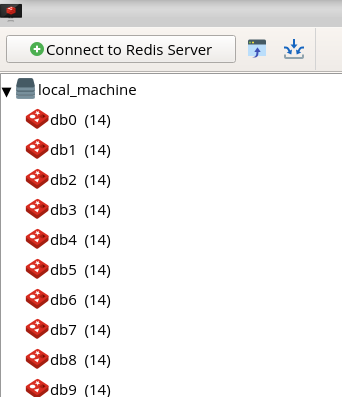
\includegraphics{1.png}
	\caption{}
\end{figure}

\begin{figure}[H]
	\centering
	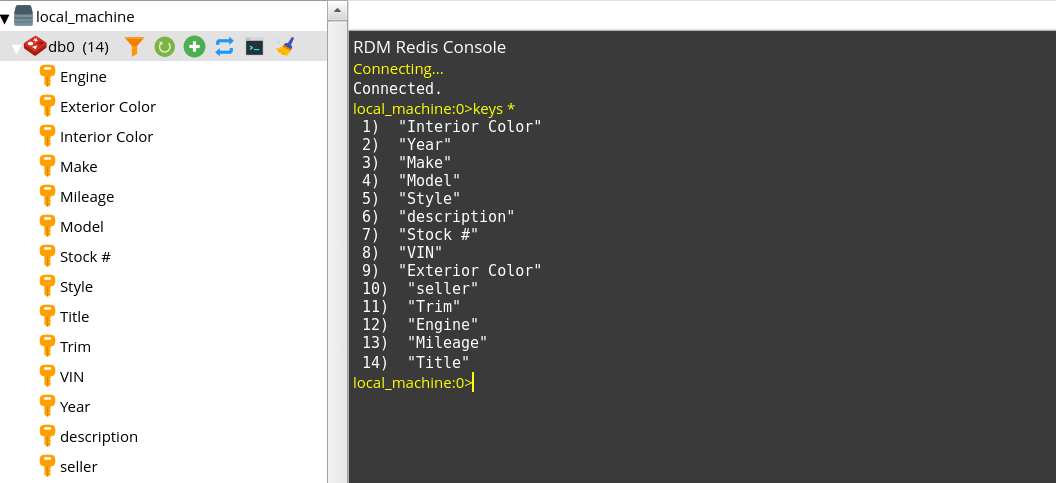
\includegraphics{2.png}
	\caption{}
\end{figure}

    \paragraph{Data model design}\label{data-model-design}

    \begin{itemize}
\tightlist
\item
  Attributes

  \begin{itemize}
  \tightlist
  \item[*]
    Title
  \item[*]
    Year
  \item[*]
    Engine
  \item[*]
    Exterior Color
  \item[*]
    Interior Color
  \item[*]
    Make
  \item[*]
    Mileage
  \item[*]
    Model
  \item[*]
    Stock
  \item[*]
    Style
  \item[*]
    Trim
  \item[*]
    VIN
  \item[*]
    Description
  \item[*]
    Seller

    \begin{itemize}
    \tightlist
    \item[*]
      address
    \item[*]
      phone
    \end{itemize}
  \end{itemize}
\end{itemize}

The data model covers all basic attributes of a car that could be found
on the retail website and that buyers should be aware of.

    \paragraph{Display sample results}\label{display-the-result}



    \begin{Verbatim}[commandchars=\\\{\}]
{\color{incolor}In [{\color{incolor}279}]:} \PY{k}{for} \PY{n}{idx} \PY{o+ow}{in} \PY{n+nb}{range}\PY{p}{(}\PY{l+m+mi}{3}\PY{p}{)}\PY{p}{:}
              \PY{n}{r} \PY{o}{=} \PY{n}{redis}\PY{o}{.}\PY{n}{StrictRedis}\PY{p}{(}\PY{n}{host}\PY{o}{=}\PY{l+s+s1}{\PYZsq{}}\PY{l+s+s1}{localhost}\PY{l+s+s1}{\PYZsq{}}\PY{p}{,} \PY{n}{port}\PY{o}{=}\PY{l+m+mi}{6379}\PY{p}{,} \PY{n}{db}\PY{o}{=}\PY{n}{idx}\PY{p}{)}
              \PY{k}{for} \PY{n}{key} \PY{o+ow}{in} \PY{n}{r}\PY{o}{.}\PY{n}{keys}\PY{p}{(}\PY{p}{)}\PY{p}{:}
                  \PY{n}{key} \PY{o}{=} \PY{n}{key}\PY{o}{.}\PY{n}{decode}\PY{p}{(}\PY{l+s+s2}{\PYZdq{}}\PY{l+s+s2}{utf\PYZhy{}8}\PY{l+s+s2}{\PYZdq{}}\PY{p}{)}
                  \PY{k}{try}\PY{p}{:}
                      \PY{n}{value} \PY{o}{=} \PY{n}{r}\PY{o}{.}\PY{n}{get}\PY{p}{(}\PY{n}{key}\PY{p}{)}
                  \PY{k}{except} \PY{n+ne}{Exception} \PY{k}{as} \PY{n}{e}\PY{p}{:}
                      \PY{n}{value} \PY{o}{=} \PY{n}{r}\PY{o}{.}\PY{n}{hgetall}\PY{p}{(}\PY{n}{key}\PY{p}{)}
                  \PY{n+nb}{print}\PY{p}{(}\PY{n}{key}\PY{p}{,}\PY{l+s+s1}{\PYZsq{}}\PY{l+s+s1}{ : }\PY{l+s+s1}{\PYZsq{}}\PY{p}{,} \PY{n}{value}\PY{p}{)}
              \PY{n+nb}{print}\PY{p}{(}\PY{l+s+s1}{\PYZsq{}}\PY{l+s+se}{\PYZbs{}n}\PY{l+s+s1}{\PYZsq{}}\PY{p}{)}
\end{Verbatim}

    \begin{Verbatim}[commandchars=\\\{\}]
Interior Color  :  b'Black'
Year  :  b'2014'
Make  :  b'Subaru'
Model  :  b'Outback'
Style  :  b'Sport Utility'
description  :  b"CARFAX One-Owner. Clean CARFAX. Blue 2014 Subaru Outback 2.5i Premium AWD 6-Speed 2.5L 4-Cylinder DOHC 16VWe at Stocker Chevrolet appreciate your time and understand you have better things to do than shop for a new Chevrolet. That's why we price our online vehicles well below market averages! We want you to feel confident your not overpaying when you purchase your new Chevrolet at Stocker Chevrolet. Come in today and see why Stocker Chevrolet is the fastest growing Chevrolet dealerships in PA!Awards:* 2014 KBB.com 10 Best All-Wheel-Drive Cars \& SUVs Under \$25,000Call or email today to make an appointment with one of our GREAT GREAT sales professionals who will show you how easy it is to buy your new Chevrolet from Stocker Chevrolet!Reviews:* Need a lot of interior room? Reasonable fuel economy? Rugged durability? All-weather capability? Good results on crash tests? And all that at an affordable price? The 2014 Outback should be high on your list. Source: KBB.com* Spacious interior; comfortable ride; excellent visibility; clever roof rails; above average off-road capability. Source: Edmunds* The 2014 Subaru Outback has what you need to explore whenever and wherever with confidence. The 2014 Subaru Outback now comes standard with adaptive transmission control with a continuously variable automatic transmission. The optional nav system also now includes a multimedia system with smartphone integration. With Subaru Symmetrical All-Wheel Drive and a rugged suspension, you get car-like handling with SUV capabilities. Outback is available with an innovative driver-assist system: EyeSight, a combination of four systems that help the driver watch for and avoid trouble ahead. Choose the 173-hp 2.5-liter 4-cylinder SUBARU BOXER engine and a refined Lineartronic CVT combine to get up to 30 highway MPG. Or opt for the 256-hp 3.6-liter 6-cylinder SUBARU BOXER engine. The Outback is smartly equipped with retractable and adjustable cross bars, ample cargo room, and an array of places to store, stash, secure, hook up and tie-down. The spacious cabin and clever designs found on every Outback make getting in, getting out and getting all of your gear easier for you and your passengers. Generous legroom in the back, plenty of hip room in the front and spacious headroom all around make everyone comfortable with plenty of room for plenty of stuff. Fold down the 65/35 split seats and you can boost your cargo capacity to more than 71 cubic feet when big plans call for big things. Outback offers the latest in technology. Standard Bluetooth connectivity, steering-wheel-mounted controls, voice activated 7-inch touch screen GPS navigation system, NavTraffic, rear-vision camera, auto-dimming rearview mirror with HomeLink, power tilt/sliding-glass moonroof, windshield wiper de-icer, heated side mirrors, heated front seats, and a 440-watt 9-speaker Harman Kardon premium audio system with amplifier and subwoofer, HD Radio, USB port iPod control, and SiriusXM satellite radio. Source: The Manufacturer Summary"
Stock \#  :  b'606614A'
VIN  :  b'4S4BRBCC4E3219562'
Exterior Color  :  b'Twilight Blue Metall'
seller  :  \{b'address': b' 701 Benner Pike State College PA, 16801 ', b'phone': b'(866) 235-0270'\}
Trim  :  b'2.5i Premium'
Engine  :  b'4 -'
Mileage  :  b'75655'
Title  :  b'2014 Subaru Outback'


Interior Color  :  b'Black'
Year  :  b'2013'
Make  :  b'Subaru'
Model  :  b'XV Crosstrek'
Style  :  b'Station Wagon'
description  :  b"Clean CARFAX. Orange 2013 Subaru XV Crosstrek 2.0i Premium AWD 5-Speed Manual 2.0L 16V DOHCWe at Stocker Chevrolet appreciate your time and understand you have better things to do than shop for a new Chevrolet. That's why we price our online vehicles well below market averages! We want you to feel confident your not overpaying when you purchase your new Chevrolet at Stocker Chevrolet. Come in today and see why Stocker Chevrolet is the fastest growing Chevrolet dealerships in PA! Odometer is 4798 miles below market average! 30/23 Highway/City MPGAwards:* 2013 IIHS Top Safety PickCall or email today to make an appointment with one of our GREAT GREAT sales professionals who will show you how easy it is to buy your new Chevrolet from Stocker Chevrolet!Reviews:* Today's small-SUV shopper faces no shortage of choices, but if all-terrain capability and distinctive exterior styling are prerequisites for your next compact SUV, the 2013 XV Crosstrek should make your decision much easier. Source: KBB.com"
Stock \#  :  b'204842B'
VIN  :  b'JF2GPACCXD1843307'
Exterior Color  :  b'Tangerine Orange Pea'
seller  :  \{b'address': b' 701 Benner Pike State College PA, 16801 ', b'phone': b'(866) 235-0270'\}
Trim  :  b'Premium'
Engine  :  b'4 -'
Mileage  :  b'69331'
Title  :  b'2013 Subaru XV Crosstrek'


Interior Color  :  b'Jet Black/Medium Tit'
Year  :  b'2014'
Make  :  b'Chevrolet'
Model  :  b'Cruze'
Style  :  b'4dr Car'
description  :  b"CARFAX One-Owner. Clean CARFAX. Blue 2014 Chevrolet Cruze LS FWD 6-Speed Automatic Electronic with Overdrive ECOTEC 1.8L I4 SMPI DOHC VVTWe at Stocker Chevrolet appreciate your time and understand you have better things to do than shop for a new Chevrolet. That's why we price our online vehicles well below market averages! We want you to feel confident your not overpaying when you purchase your new Chevrolet at Stocker Chevrolet. Come in today and see why Stocker Chevrolet is the fastest growing Chevrolet dealerships in PA! Recent Arrival! 35/22 Highway/City MPGAwards:* 2014 KBB.com Brand Image AwardsCall or email today to make an appointment with one of our GREAT GREAT sales professionals who will show you how easy it is to buy your new Chevrolet from Stocker Chevrolet!Reviews:* The Cruze stands out from other compacts with its comfort-oriented ride and overall feeling of solidity and strength. If you've been yearning for a powerful, high-mileage diesel compact sedan, the Chevrolet Cruze Clean Turbo Diesel is the only such vehicle available for 2014 besides Volkswagen's Jetta. Source: KBB.com* Handsome interior design; two satisfying high-efficiency engine choices; useful electronics interface; secure handling; big trunk. Source: Edmunds* The 2014 Cruze gives you great fuel economy and a reasonable price, with a very stylish look to go with it. It has a strong stance and angled lines, with a split front grille, and headlights that wrap around from the front and end in a point above the fenders. On the inside the cabin is modern, roomy and comfortable. It doesn't feel like the compacts you might be used to and is refreshingly fun to drive. There are 6 different trims available for the 2014 Cruze, including the: LS, 1LT, eco, 2LT, LTZ, and the Diesel. Standard for all are features such as Air Conditioning, Power Windows and Door Locks, Power Steering and Touch Controls on the Steering Wheel. The Base Model LS comes with a 1.8-liter, 4-Cylinder engine that gets an EPA estimated 25MPG City and 36MPG hwy with the standard 6-speed manual, or 22MPG City and 35MPG Highway when you opt for the available automatic. All models higher than the LS, but below the Diesel come with a peppy 1.4-Liter, 4-Cylinder Turbocharged Engine. The 1LT and 2LT give you your choice of a 6-speed manual with overdrive or an automatic. The Eco comes standard with a special 6-speed manual with triple overdrive, or an optional automatic. The LTZ however only comes with an Automatic transmission. Fuel economy varies for these four trims based on which transmission you opt for, but the best performer hands down is the Eco with the Manual Transmission that gets an EPA estimated 28MPG City and 42MPG highway. The top of the line model is the Diesel. It has a 2.0-liter, 4-Cylinder engine that has 148 Horsepower, and gets an EPA estimated 27MPG in the City and an amazing 46MPG on the Highway. All that without the stinky fumes you might be used to from diesels of the past. Standard safety features on all models include Anti-lock brakes, Stabilitrak, Traction Control, and 10 Airbags. Upgrade to the LTZ trim and you get the added visibility of a Rear View Camera. Come drive the 2014 Chevrolet Cruze Today! Source: The Manufacturer Summary"
Stock \#  :  b'204275A'
VIN  :  b'1G1PA5SG4E7343131'
Exterior Color  :  b'Atlantis Blue Metall'
seller  :  \{b'address': b' 701 Benner Pike State College PA, 16801 ', b'phone': b'(866) 235-0270'\}
Trim  :  b'LS'
Engine  :  b'4 -'
Mileage  :  b'61147'
Title  :  b'2014 Chevrolet Cruze'


    \end{Verbatim}

    
    

    % Add a bibliography block to the postdoc
    
    
    
    \end{document}
